\chapter{Clean Architecture}

\section{Was ist Clean Architecture?}
Die \textit{Clean Architecture} ist ein Gestaltungskonzept, das darauf
abzielt möglichst robuste und wartbare Anwendungen zu entwickeln. Dabei
wird eine Software in hierarchisch mehrere Schichten organisiert, was
gemeinhin als \textit{Onion-Architektur} bekannt ist. Jede Schicht
weist dabei eine spezifische Verantwortung (siehe \textit{domain}, 
\textit{plugins} etc.). 

Die Schichten sind über Schnittstellen verbunden. Hinter den
Schnittstellen steckt dann eine tatsächliche Implementation. Ziel ist
es dadurch eine Trennung zwischen der Logik einer Schicht und den
technischen Details einer anliegenden Schicht zu erzeugen. Statt durch
konkrete Implementierungsdetail sind die Schichten (zumindest von innen
nach außen) über
Funktionsabmachungen in Form der Schnittstellen verbunden. Dadurch
lassen sich leicht Änderungen in einer Schicht vornehmen, ohne dabei
zwangsläufig Änderungen in einer anderen Schicht vornehmen zu müssen.

Entscheidend für das Prinzip ist die Abhängigkeitsrichtung. Äußere
abstraktere Schichten (hierarchisch untergeordnet) können direkt auf
innere Schichten zugreifen und von ihnen abhängig sein. Jedoch gilt
dies nicht für die Umkehrrichtung. Aufrufe von innen nach außen werden
über Schnittstellen und Abstraktionen sichergestellt 
(\textit{Dependency Inversion} und \textit{Injection}).
Tieferliegende Schichten sind zudem am wenigsten abstrakt und damit
am langlebigsten.

Dieser Sachverhalt führt zu Anwendungen, die wartbarer und robuster sind,
weil Änderungen an einer Schicht meist keine Änderungen an anderen
Schichten verursachen. Durch clevere Trennung und Abstraktionen lässt
sich der Anpassungaufwand durch eine beliebige Änderung an vielen Stellen
einsparen.

\section{Analyse der Dependency Rule}
Die Schichten der \textit{Onion-Architektur} sind sortiert von innerster
nach äußerster Schicht \textit{abstraction}, \textit{domain},
\textit{application} und \textit{plugin}. Es sind lediglich Abhängigkeiten
von außen nach innen erlaubt, aber nicht umgekehrt. Die Schichten sind
in einzelne Module gegliedert. Diese haben andere Module, also andere
Schichten als fest definierte Import-Möglichkeiten. Dadurch wird
sichergestellt, das eine Schicht auch nur von unterliegenden Schichten
abhängig sein kann. Sollte eine Abhängigkeit nach außen bestehen, so
kann das Programm nicht gebaut werden, weil Imports fehlen.

\pagebreak
\subsection*{Positiv-Beispiel I}
Die nachfolgende Abbildung zeigt ein vereinfachtes UML-Diagramm der
Klasse \textit{GridPosition} und die Abhängigkeiten in beide Richtungen.
Die Klasse stammt aus der Schicht \textit{application}.
Wie zu sehen, hängt \textit{GridPosition} lediglich von den Klassen
\textit{Position} und \textit{IVectorizable} aus den jeweilig 
unterliegenden Schichten \textit{domain} und \textit{abstraction} ab.
Weiterhin ist zu sehen, dass nur Klassen der gleichen Schicht
(\textit{application}) von \textit{GridPosition} abhängen, jedoch
keine Klasse aus einer tieferen Schicht (weiter innen liegend, z.B.
\textit{abstraction} oder \textit{domain}). Dadurch ist die
\textit{Dependency Rule} gewahrt.

\vspace{0.5cm}
\begin{figure}[H]
    \centering
    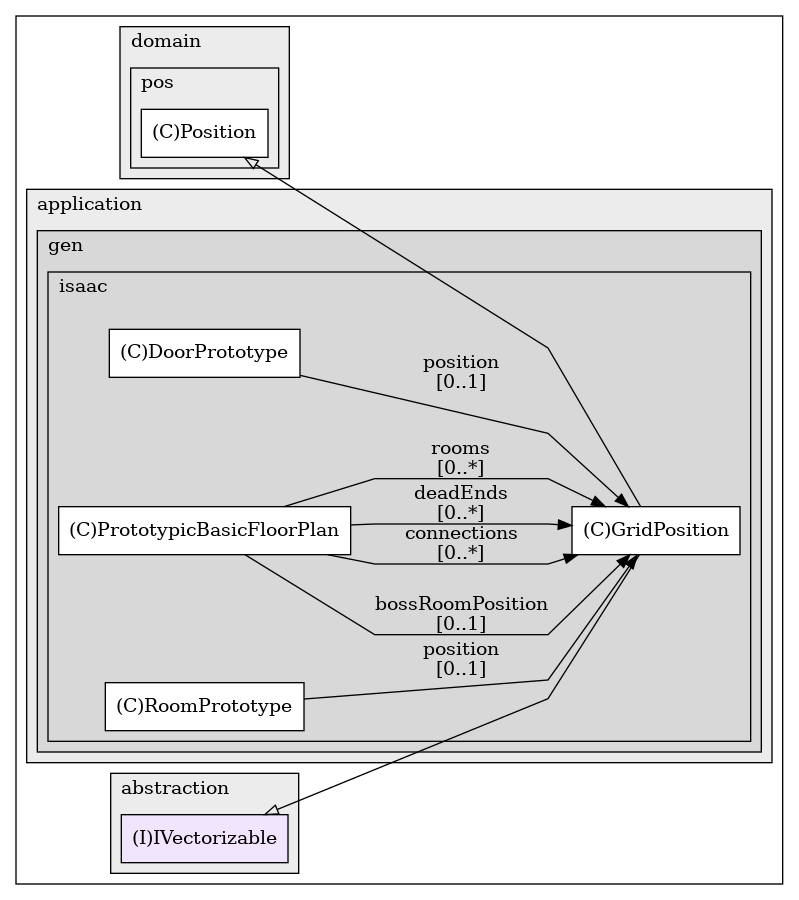
\includegraphics[width=0.8\linewidth]{Bilder/Visualisierung/GridPosition_structure.png}
    \caption{Dependency Rule I: GridPosition}
\end{figure}

\subsection*{Positiv-Beispiel II}
Die nachfolgende Abbildung zeigt ein vereinfachtes UML-Diagramm der
Klasse \textit{Player} und die Abhängigkeiten in beide Richtungen.
Die Klasse stammt aus der Schicht \textit{domain}.
Es ist zu sehen, dass \textit{Player} von einigen Klassen der gleichen
Schicht wie etwa \textit{LivingEntity},  \textit{Level} und \textit{Item}
abhängt. Darüber hinaus hängt die Klasse \textit{Room} von der Klasse
\textit{Player} ab. Interessant ist allerdings, dass die Klasse
\textit{GameState} aus der höherliegenden Schicht \textit{application}
von \textit{Player} abhängt. Die Abhängigkeitsrichtung zeigt von 
außen nach innen, verletzt also die \textit{Dependency Rule} nicht.
Die Klasse \textit{Player} hängt jedoch noch von einem Interface
names \textit{IGlobalState} ab, welches von \textit{GameState}
implementiert wird. Das Interface stellt daher eine Schnittstelle
zwischen \textit{domain} und \textit{application} dar, durch welche
der \textit{Player} mit konkreten Implementationen von \textit{IGlobalState}
in höherliegenden Schichten, wie etwa \textit{GameState}, kommunizieren
kann, ohne von ihnen abhängig zu sein. Dies ist ein wichtiges Merkmal
der \textit{Clean Architecture}.

\vspace{0.5cm}
\begin{figure}[H]
    \centering
    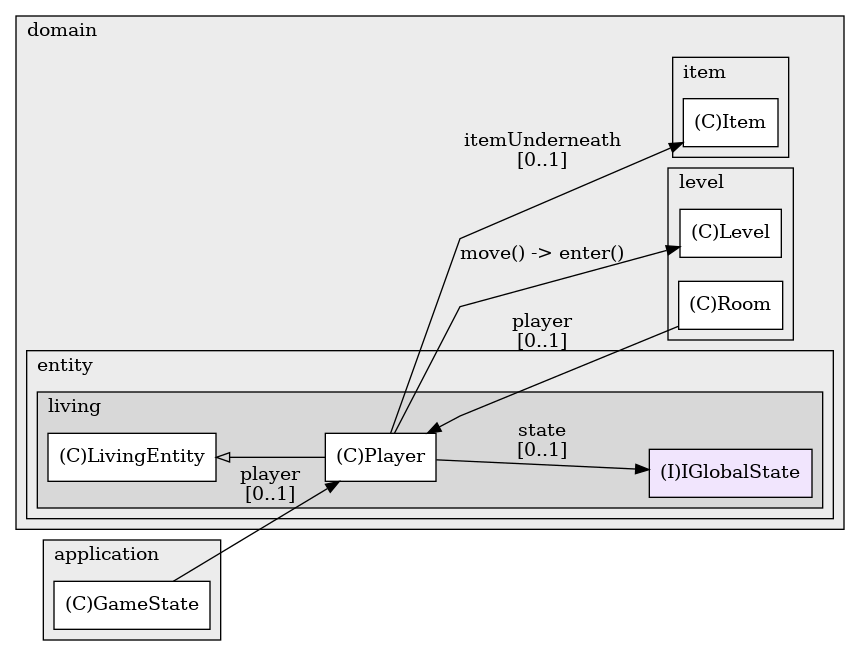
\includegraphics[width=0.9\linewidth]{Bilder/Visualisierung/Player_structure.png}
    \caption{Dependency Rule II: Player}
\end{figure}

\section{Analyse der Schichten}
\subsection*{Domain Schicht}
Die Klasse \textit{Room} ist ein integraler Bestandteil des Spiels
(Domäne) und ist daher in der \textit{domain} Schicht integriert. Eine
Umsiedlung in eine andere Schicht ist nicht sinnvoll. Wie der
nachfolgenden Grafik zu entnehmen ist, hängt sie sehr stark mit
anderen Klassen der Domäne wie etwa \textit{Item}, \textit{Level},
\textit{Door} oder \textit{Entity} zusammen. Dies unterstreicht die
Bedeutung in der Domäne und legitimiert die Einordnung. Ihre Aufgabe
ist die modellhafte Abbildung eines Level-Raumes und dessen Verwaltung.
Dabei hält es alle enthaltenen Gegner, den Spieler und Items vor. Zudem
ist dem Raum auch bewusst, ob er bereits betreten wurde und ob er von
Gegnern befreit wurde. Wurde der Raum noch nicht betreten, so werden
Gegner beschworen. Ist er noch nicht komplett von Gegner befreit, 
hindert er den Spieler am Fliehen. Zudem stellt es einige Helferfunktionen
bereit, wie etwa \textit{getClosestEnemy()}, da es umfangreiches Wissen
über den Zustand des Raumes beinhaltet.

\vspace{0.5cm}
\begin{figure}[H]
    \centering
    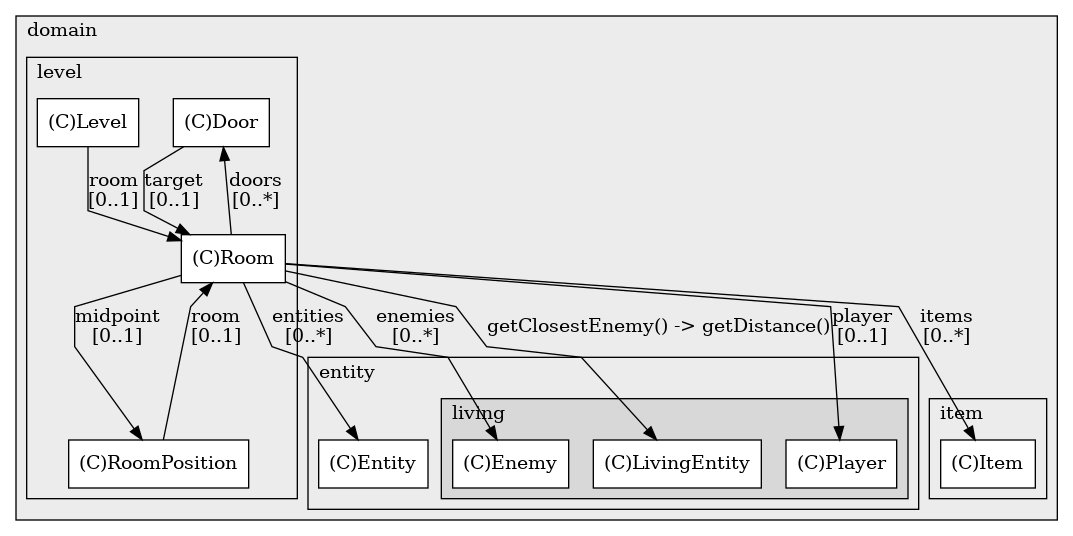
\includegraphics[width=0.9\linewidth]{Bilder/Visualisierung/Room_structure.png}
    \caption{Analyse der Schichten: Domain}
\end{figure}

\subsection*{Plugin Schicht}
Die Klasse \textit{TerminalInterface} ist ein integraler Bestandteil
der Anzeige bzw. Ausgabe und ist daher in der \textit{plugin} Schicht
integriert. Eine Umsiedlung in eine andere Schicht ist nicht sinnvoll.
Die Klasse \textit{TerminalInterface} ist ein Kompositum, welches
sich aus mehreren visuellen Komponenten (\textit{ItemView}, 
\textit{StateView} und \textit{LevelView}) zusammensetzt. Diese lesen
Spiel-Informationen aus und wandeln sie in eine passende Darstellung
um. In diesem Fall, wird in Zeichen-Buffer (siehe Klasse \textit{Buffer}
und \textit{CompositeBuffer}) gerendert. Komposita sind üblich für die
Erstellung von hierarchischen Anzeigen, welche sich üblicherweise in
der äußersten Schicht befinden. Dies untermauert die Einordnung in die
\textit{plugin} Schicht. Zudem hängt keine andere Klasse, nicht einmal
über ein Interface, von \textit{TerminalInterface} ab. Das 
\textit{TerminalInterface} selbst hängt wiederum von einem Interface
namens \textit{IInterface} ab, welches lediglich zur Orchestrierung
einer Anzeige dient und \textit{render()}-Befehle absetzt. Es ist
daher sehr leicht auszutauschen durch eine andere Anzeige-Mechanik.
Dies ist typisch für \textit{Plugins}.

\vspace{0.5cm}
\begin{figure}[H]
    \centering
    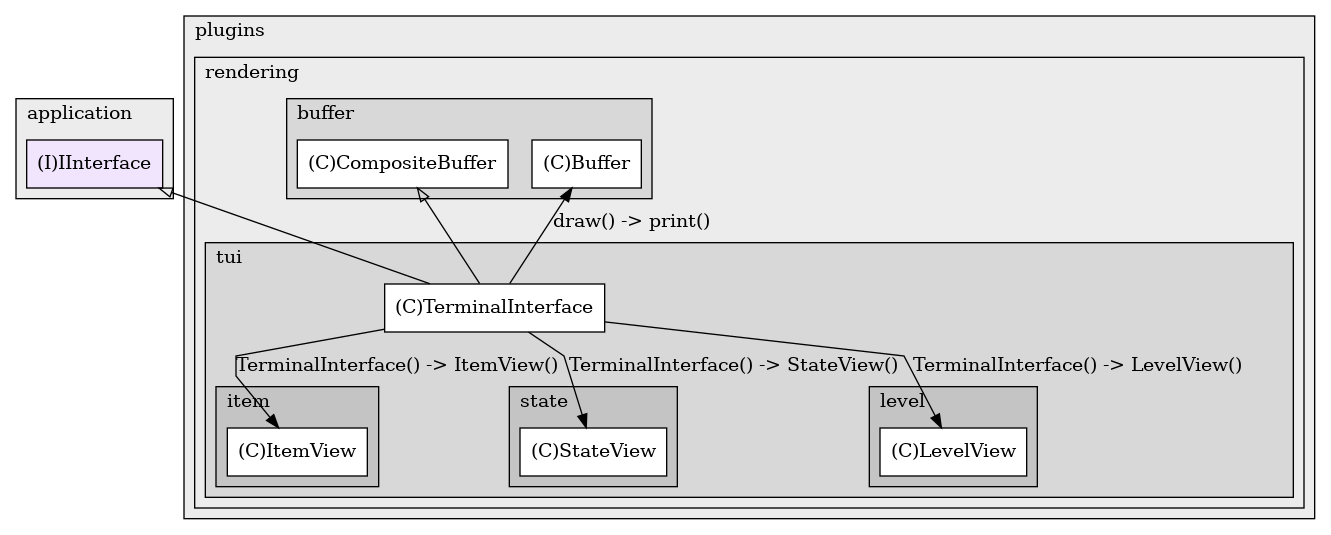
\includegraphics[width=0.9\linewidth]{Bilder/Visualisierung/TerminalInterface_structure.png}
    \caption{Analyse der Schichten: Plugin}
\end{figure}